% !TEX TS-program = pdflatex
% !TEX encoding = UTF-8 Unicode 
\documentclass[a4paper,11pt,openright,BCOR=15mm]{scrbook}

\usepackage[onehalfspacing]{setspace}    %   
\usepackage[utf8]{inputenc}
\usepackage[portuges,english]{babel}     
\usepackage[square,numbers]{natbib}
\usepackage{graphicx}               
\usepackage[pdftex]{hyperref}
\usepackage[T1]{fontenc}          
\usepackage{pdfpages}         
\usepackage{lettrine}    
\usepackage{booktabs}  
\usepackage{scrhack}   
\usepackage{scrlayer-scrpage}
\usepackage{ulem} % for underline
\usepackage{xcolor}
\definecolor{cinza1}{RGB}{200,200,200}
\definecolor{cinza2}{RGB}{70,70,70}
\usepackage{vhistory}	%% para versoes....
\newcommand\ChapterFont{}      % usar o tipo de letra normal
\newcommand\SectionFont{}
\pagestyle{scrheadings}
\ifoot[]{\raisebox{-32pt}{
\includegraphics[width=0.15\textwidth]{logos/logoisep}}}
\ofoot[]{\raisebox{-22pt}{
\includegraphics[width=0.10\textwidth]{logos/logo_DEI_big_transparente}}}
\cfoot[\pagemark]{\pagemark}
\automark[section]{chapter}
\usepackage{blindtext}   % \texto para demos 
\usepackage{listings}   %  para listagens com diferentes tipos de letra
\usepackage{fancyvrb}  %  para listagens de codigo 
\usepackage{float}
%%%%%%%%%%%%%%%%%%%%%%%%%%%%%%%%%%%%%%%%%%%%%%%%%%%%%%%%%%%%%%%%%%%%%%%%%%%%
\usepackage[mono=false]{libertine}
%%%%%%%%%%%%%%%%%%%%%%%%%%%%%%%%%%%%%%%%%%%%%%%%%%%%%%%%%%%%%%%%%%%%%%%%%%%%%%%%%%%%%%%%%
\begin{document}
	
	\selectlanguage{english}  
	\frontmatter
	
	\titlehead{
\includegraphics[scale=0.2]{figs/logoisep}
		\hfill 
\includegraphics[scale=0.115]{logos/logo_DEI_big_transparente}
	}  
	
	\title{Project (Second Part) \\ \underline{Global report of group 200} 
		}
	\subtitle{QSOFT}
	
	\author{Master in Informatics Engineering - 2024/2025}        
	
	
\publishers
{
	1181180, \\1191526, \\1201100, \\1230210,\\1240485\\    \texttt{Version \vhCurrentVersion, \vhCurrentDate}\\
}         
  
	
	
	
	\date{Porto, \today} 
	
	
	\maketitle   
	
	\begin{versionhistory}
		\vhEntry{1}{2024-11-26}{Group 200}{Initial Version}  
		\vhEntry{2}{2024-12-02}{Group 200}{Final Version}  
	\end{versionhistory}
	
	\cleardoublepage
	

	
	
	
	\tableofcontents
	\addcontentsline{toc}{chapter}{List of Figures}
	\listoffigures
	
	
	
	% \listoftables 
	
	\mainmatter 
	
	%% =================================
	
	
	%% =================================
	\chapter{Introduction}
	
	This document details the work completed by Group 200 as part of the "Software Quality" course within the Master's program in Informatics Engineering at Instituto Superior de Engenharia do Porto (ISEP). The main focus of the project was to assess the "PetClinic" application, examining its quality to determine if it meets the necessary criteria for reuse in other projects. The report is organized into different sections, including the project context, team responsibilities, technologies employed, established conventions, the Goal-Question-Metric (GQM) framework, and the final conclusions drawn from the analysis.
	
	\chapter{Context}	
		\section{Project generation - JHipster}	
		The application’s source code was generated using the JHipster tool. Upon installation, we configured the base project based with JWT token and SQL Server database (the other configuration are not to important for here). Once the initial application was generated, we proceeded to define the core structure by identifying entities: Pet, PetType, Vet, Visit and Owner. These entities, along with their relationships, were detailed in a JDL (JHipster Domain Language) file named \textit{modelo.jdl}, which was saved in the project repository. This file acted as a detailed blueprint for the domain model, specifying the structure and interconnections of the various entities.
		
		To generate the source code for each aggregate, we used the command \textit{jhipster import-jdl modelo.jdl}. Following this, running the command ./mvnw started the application, as shown in figure \ref{fig:Domain JDL Diagram}. Each aggregate was designed with the core CRUD (Create, Read, Update, Delete) operations in mind, ensuring a cohesive and seamless user experience. 
			
		\begin{figure}[H]
			\begin{center}
				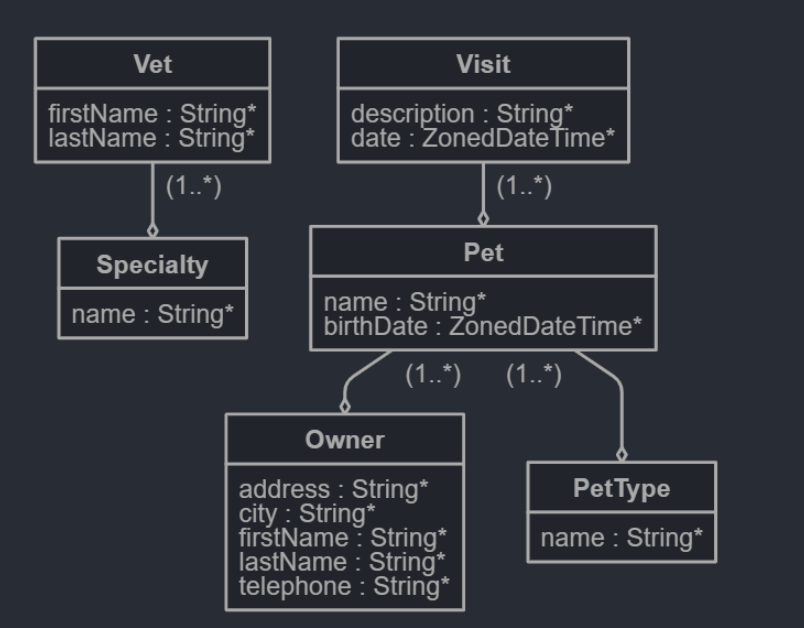
\includegraphics[width=\textwidth]{figs/JDL.png}
				\caption{Domain JDL Diagram}
				\label{fig:Domain JDL Diagram}
				\centering
			\end{center}
		\end{figure}
		
		\section{Architecture}
		
		The architecture of an application generated by JHipster, with \textbf{Angular} for the frontend and \textbf{SQL Server} as the database.
		JHipster typically generates a layered architecture that divides the application into distinct layers, each with its own responsibilities. This modular approach ensures scalability, maintainability, and clear boundaries between different parts of the application.
		
		\subsection{Frontend - Angular}
		The frontend is built with Angular, a powerful JavaScript framework that enables the creation of dynamic, single-page applications (SPA). Angular follows a component-based architecture, where the UI is divided into small, reusable components. These components interact with services that handle business logic, data fetching, and communication with the backend.
		
		\begin{enumerate}
			\item \textbf{Components:} Angular components define the structure and logic of the user interface. They manage user input, display data, and handle interactions.
			\item \textbf{Services:} Angular services provide methods to interact with the backend and handle business logic. They are responsible for making HTTP requests to the Spring Boot API, managing application state, and handling data processing.
			\item \textbf{Modules:} Angular modules group related components, services, and other elements, providing a logical organization of the frontend application.
		\end{enumerate}
		
		\subsection{Backend  - Spring Boot}
		On the backend, JHipster generates a Spring Boot application, which is a widely used framework for building Java-based, production-grade web applications. Spring Boot simplifies the development of RESTful APIs and integrates seamlessly with various databases, including \textbf{SQL Server}.
		
		\begin{enumerate}
			\item \textbf{Controllers:} Spring Boot uses controllers to handle incoming HTTP requests from the frontend. These controllers map requests to appropriate service methods and return data to the client in JSON format.
			\item \textbf{Services:} Service classes in Spring Boot encapsulate the business logic of the application. They interact with repositories to retrieve and manipulate data and perform necessary operations before sending a response to the client.
			\item \textbf{Repositories:} The repository layer in Spring Boot provides an abstraction for database operations, and JHipster uses Spring Data JPA to automatically generate the necessary database queries based on the entities defined in the application.
		\end{enumerate}
		
		\subsection{Database - SQL Server}
		The application uses SQL Server as the relational database management system. JHipster generates the necessary configuration to connect Spring Boot with SQL Server, and entities are defined using JPA (Java Persistence API) annotations. This allows the application to perform CRUD operations on the database seamlessly.
		
		\begin{enumerate}
			\item \textbf{Entities:} The JHipster generator creates entities that represent tables in the SQL Server database. Each entity maps to a specific business domain and contains fields that correspond to the table’s columns.
			\item \textbf{Database Migrations:} JHipster provides Liquibase for database version control, ensuring that schema changes are managed and synchronized across different environments.
		\end{enumerate}
		
		\subsection{Monolithic Architecture}
		The entire application is packaged as a single deployable unit. The frontend and backend share the same codebase, and the application is typically easier to deploy and manage initially. This approach works well for small to medium-sized applications that do not require independent scaling of components.
		
		\subsection{Securiy and Authentication}
		The application is secured with \textit{JWT}, which provides token-based authentication for stateless communication between the frontend and backend.
		
		\section{Conventions}
		
		The project follows a set of conventions to ensure consistency and readability in the
		project. Some of the detected conventions are:
		
		\begin{enumerate}
			\item URL Structure: Base Path starts with /api/{entity}
			\item CRUD Operations :
			\begin{enumerate}
				\item GET : /api/{entity} -> Get all entity objects
				\item GET : /api/{entity}/{id} -> Get the entity filtered by id
				\item POST : /api/{entity} -> Creates a new object
				\item PUT : /api/{entity}/{id} -> Updates the object containing the specific ID
				\item DELETE : /api/{entity}/{id} -> Deletes a specific ID
			\end{enumerate}
			\item Authorization based in JWT
		\end{enumerate}
	
	%% =================================
	
	\chapter{Work distribution}
	This chapter describes the assignments of each student, as follows:\newline
		
		\begin{itemize}
			\item Student 1181180 - Owner Aggregate: 
			\begin{itemize}
				\item Accessibility : Used Lighthouse and WAI Statement Generator
				\item Visual Compatibility : BackstopJS in login and Main pages
				\item Maintainability : Number of Java Packages and The Cumulative Component Dependency (CCD)
				\item Performance : 
				\begin{itemize}
					\item JMeter and K6 for Load, Stress and Soak test (PUT + GET)
					\item Lighthouse for Frontend Performance (RAIL metrics)
				\end{itemize}	
				\item Security : 
				\begin{itemize}
					\item Dependency Vulnerabilities with Dependency Checker Plugin
					\item Check A05 and A06 from OWASP Top 10 using OWASP ZAP
				\end{itemize}	
			\end{itemize}
			\item Student 1191526 - Vet Aggregate: 
			\begin{itemize}
				\item Accessibility : Used Lighthouse and WAI Statement Generator
				\item Visual Compatibility : BackstopJS
				\item Maintainability :  Coupling and Structural Erosion: Maintainability Level;
				Size and Complexity: Number of Types; Instability and Cyclomatic Complexity
				\item Performance : 
				\begin{itemize}
					\item JMeter and K6 for Load, Stress and Soak test (PUT + GET)
					\item Lighthouse for Frontend Performance
				\end{itemize}	
				\item Security : 
				\begin{itemize}
					\item Dependency Vulnerabilities with Dependency
					Checker Plugin and Maven Repository
					\item Check A01 and A03 from OWASP Top 10 using OWASP ZAP
				\end{itemize}	
			\end{itemize}	
			\item Student 1201100 - Specialty Aggregate: 
			\begin{itemize}
				\item Accessibility : Used Lighthouse and WAI Statement Generator
				\item Visual Compatibility : BackstopJS
				\item Maintainability :  Coupling and Structural Erosion: Normalized Cumulative Component Dependency (NCCD);
				Size and Complexity: Number of Statements; Instability and Cyclomatic Complexity
				\item Performance : 
				\begin{itemize}
					\item JMeter and K6 for Load, Stress and Soak test (GET + POST)
					\item Lighthouse for Frontend Performance
				\end{itemize}	
				\item Security : 
				\begin{itemize}
					\item Dependency Vulnerabilities with Dependency Checker
					Async and Maven Core
					\item Check A02 and A04 from OWASP Top 10 using OWASP ZAP
				\end{itemize}	
			\end{itemize}
			\item Student 1230210 - Pet:
			\begin{itemize}
				\item Accessibility : Used Lighthouse and WAI Statement Generator
				\item Visual Compatibility : Percy
				\item Maintainability :  Coupling and Structural Erosion: Propagation Cost;
				Size and Complexity: Total Line of codes and Code Comment Lines; Instability and Cyclomatic Complexity
				\item Performance : 
				\begin{itemize}
					\item JMeter for Load, Stress and Soak test (GET)
					\item Lighthouse for Frontend Performance
				\end{itemize}	
				\item Security : 
				\begin{itemize}
					\item Dependency Vulnerabilities with Dependency
					Checker Plugin and Maven Repository
					\item Check A07 and A08 from OWASP Top 10 using OWASP ZAP
				\end{itemize}	
			\end{itemize}
			\item Student 1240485 - PetType:
			\begin{itemize}
				\item Accessibility : Used Lighthouse and WAI Statement Generator
				\item Visual Compatibility : BackstopJS on Visualise Page of PetType and List Page of PetType
				\item Maintainability: Average Component Dependency (ACD) and Number of Components/Sources
				\item Performance:
				\begin{itemize}
					\item JMeter and K6 for Load (Post), Stress (Get) and Soak (Get) test.
					\item Lighthouse for Frontend Performance
				\end{itemize}
			\end{itemize}	
		\end{itemize}
		

	
	
	%% =================================
	
	\chapter{Technologies }
	 \section{JHipster}
	 JHipster is a development platform used to generate, develop, and deploy modern web applications and microservices. It combines popular frameworks such as Spring Boot for the backend and Angular or React for the frontend. JHipster simplifies the development process by providing ready-to-use code and configurations for creating scalable, secure, and high-performance applications. It supports various features like user authentication, database integration, and deployment tools, making it ideal for building full-stack applications with minimal setup.
	 
	 
	 \section{Dependency Check plugin}
	 The Dependency Check plugin is a tool used to identify known vulnerabilities in project dependencies. It scans the libraries and frameworks included in a project and compares them against a database of publicly known security issues, such as those found in the National Vulnerability Database (NVD). By integrating this plugin into the build process, developers can automatically detect security risks in their dependencies and take corrective actions before deploying the application. This helps ensure that the project remains secure by proactively managing and updating third-party libraries to avoid potential security threats.
	 
	 \section{BackstopJS}
	 BackstopJS is an open-source testing tool used to perform visual regression testing on web applications. It helps developers ensure that changes to a website's code do not unintentionally affect its appearance. BackstopJS works by taking screenshots of web pages before and after changes, then comparing them to detect visual differences. If any discrepancies are found, the tool highlights them, allowing developers to quickly spot unintended visual changes. This is useful for maintaining consistent design and layout across different versions of an application. BackstopJS is easy to integrate into development workflows and can be used with continuous integration (CI) tools for automated testing.
	 
	 \section{Lighthouse}
	 Lighthouse is an open-source tool developed by Google to help developers improve the quality of their web applications. It provides automated audits for performance, accessibility, best practices, and Progressive Web App (PWA) compliance. Lighthouse runs a series of tests on a web page and generates a detailed report with scores and recommendations for optimization. It is commonly used to measure key performance metrics like loading speed and interactivity, offering insights into areas that need improvement to enhance user experience and ensure the site meets modern web standards.
	 
	 \section{Apache Jmeter}
	 JMeter is an open-source tool primarily used for performance and load testing web applications. It allows users to simulate multiple users accessing a system simultaneously to evaluate its behavior under stress and measure its performance, such as response times, throughput, and resource usage. JMeter can test both static and dynamic resources, making it suitable for testing web servers, databases, and other services. It provides a user-friendly interface for creating test plans, analyzing results, and generating reports, helping developers and testers identify bottlenecks and optimize application performance.
	  
	 \section{ZAP}
	 OWASP ZAP (Zed Attack Proxy) is a free, open-source tool used to find security vulnerabilities in web applications. It works by acting as a proxy between the user and the application, allowing it to monitor and analyze the communication between them. ZAP helps identify common security issues like cross-site scripting (XSS) and SQL injection by scanning the website and checking for weaknesses. It also allows users to intercept and modify traffic in real-time to spot vulnerabilities. ZAP generates reports that highlight security problems and suggests fixes, making it a valuable tool for developers and security testers looking to secure their web applications.
	 
	 \section{SonarGraph}
	 Sonargraph is a software analysis tool used to assess and improve the quality of a codebase. It focuses on identifying structural issues within the code, such as dependencies, complexity, and maintainability problems. Sonargraph provides visual representations of the code’s architecture, making it easier to spot design flaws, code smells, and potential areas for refactoring. By highlighting these issues, it helps developers maintain clean, efficient, and well-organized code. The tool also offers integration with other development processes, such as continuous integration (CI), to automatically analyze the code as changes are made, ensuring ongoing code quality.

	 \section{Percy}
	Percy is a visual testing tool used to automatically capture and compare screenshots of web pages across different browsers and devices. It helps developers ensure that the appearance of a website or application remains consistent after updates or changes. By highlighting visual differences, Percy allows teams to catch unintended design or layout issues early in the development process, making it easier to maintain a consistent user interface across various platforms.
	 
	
	%% =================================
	\chapter{Conventions }
	
	Some conventions were established to maintain the organization of the project. One of these conventions was the use of GitHub Issues to associate each commit with an issue and ensure that all commits were written in English.
	
	The following figure shows the issues used (Figure \ref{fig:githubissues}), and another figure presents the milestone under which the issues were created, including a deadline corresponding to the assignment delivery date (Figure \ref{fig:githubmilestone}).
	
	\begin{figure}[H]
		\centering
		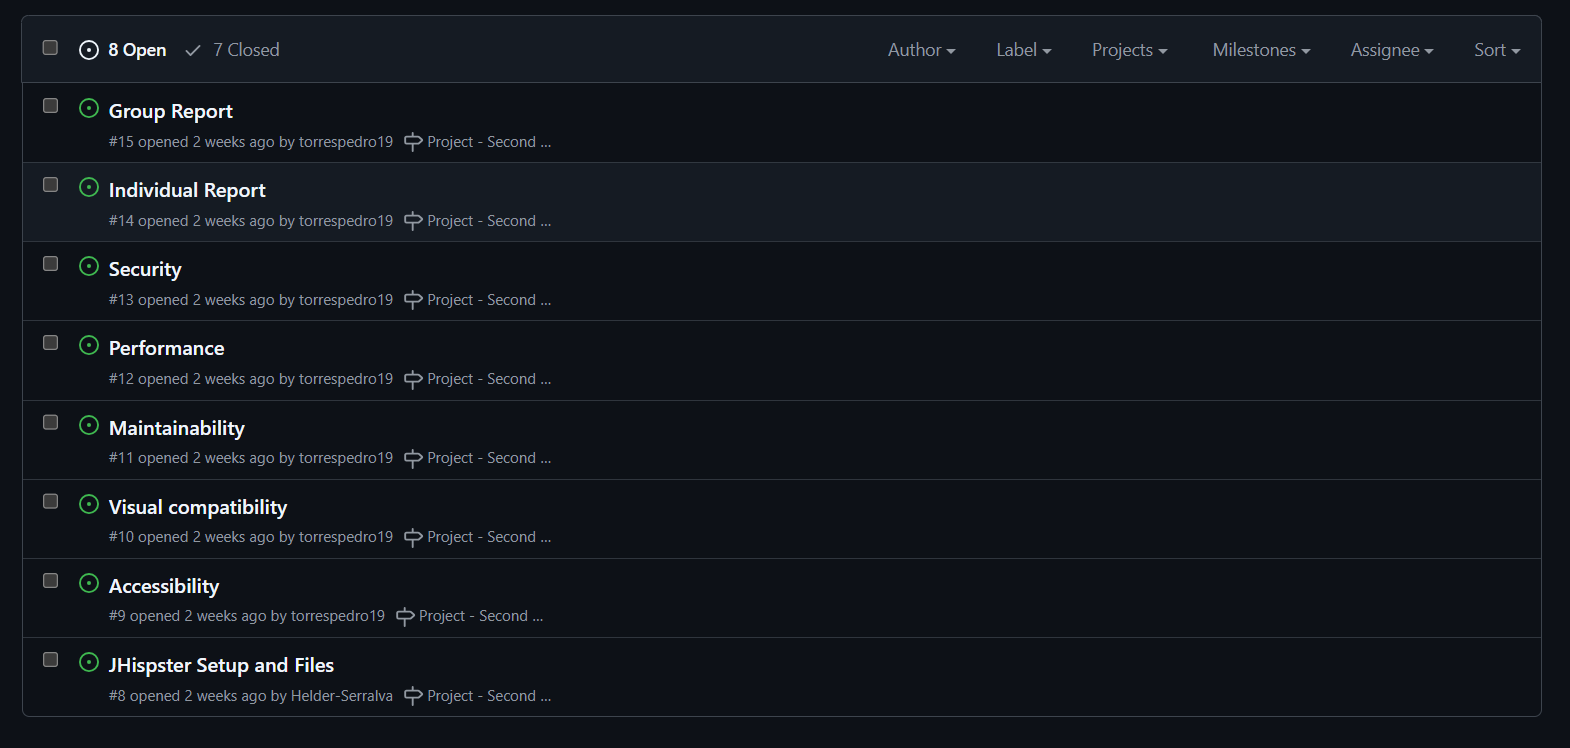
\includegraphics[width=1\linewidth]{figs/githubIssues}
		\caption{GitHub Issues}
		\label{fig:githubissues}
	\end{figure}
	
	\begin{figure}[H]
		\centering
		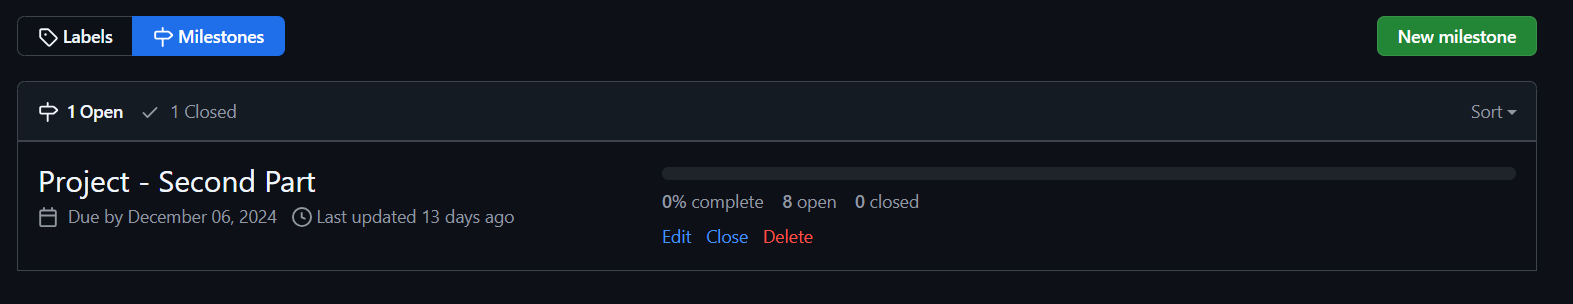
\includegraphics[width=0.7\linewidth]{figs/githubMilestone}
		\caption{GitHub Milestone}
		\label{fig:githubmilestone}
	\end{figure}
	
	As a communication channel, we used Discord to facilitate communication within the team and to stay updated on each member's progress.
	
	Finally, for documentation, we used LaTeX to create this group report. For individual reports, each member chose between LaTeX or Markdown, depending on what was more convenient.
	
	
	\chapter{Goal Question Metric (GQM)}
		
	GQM (Goal-Question-Metric) define and measure goals in software development and other fields. It involves three steps: defining Goals (what you want to achieve), deriving Questions to evaluate whether the goals are being met, and identifying Metrics to quantify the answers to these questions. This structured approach ensures alignment between objectives and measurable outcomes, improving decision-making and performance tracking.
		
	\section{Questions and Metrics}
		
	\begin{figure}[H]
		\begin{center}
			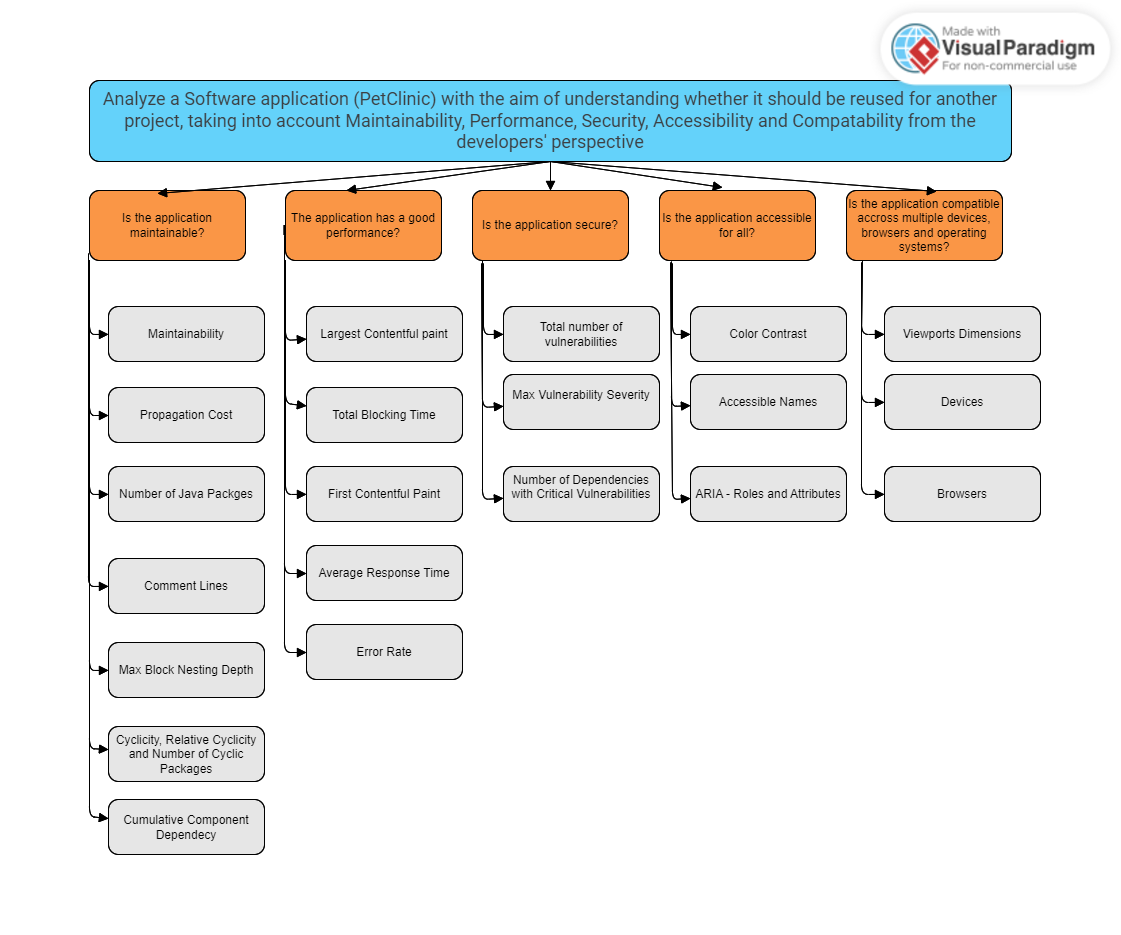
\includegraphics[width=0.85\textwidth]{figs/GQM.png}
			\caption{GQM Diagram}
			\label{fig:GQM Diagram}
			\centering
		\end{center}
	\end{figure}
	
	\pagebreak
	
	\section{Measurement scale system}
	
	Measurement, in this context, involves converting real-world observations into a formal framework to quantify the extent to which a system, component, or process exhibits a particular quality. A measure is the numerical or symbolic value assigned to represent this quality through the chosen framework. For our analysis, we will employ nominal and ordinal scales. These scales, outlined in the accompanying table, help categorize and rank data to facilitate interpretation and evaluation.
		
	\begin{table}[H]
		\centering
		\begin{tabular}{|c|c|} \hline 
			Scale& Definition\\ \hline 
			1& Very poor\\ \hline 
			2& Poor\\ \hline 
			3& Average\\ \hline 
			4& Good\\ \hline 
			5& Very Good\\ \hline
		\end{tabular}
		\caption{Measurement scale}
		\label{tab:table-scale}
	\end{table}
	
	\section{Answering questions}
	
	Each group member focused on a different aggregate, with all member also assigned to review the application as a whole. The analysis and responses presented here are based on some specific aggregates: owners, vet and pet. To determine if the application fulfills its intended purpose, we’ll now address the GQM (Goal-Question-Metric approach).
	
	\subsection{Is the application maintainable?}				
	In this new project, we achieved significantly better results in the Maintainability metrics compared to Part 1. While the individual reports suggest some areas for potential improvement, we believe the level of maintainability is more than adequate. Therefore, we have assigned a score of \textbf{5/5}.
	
	\subsection{The application maintainable has good performance?}			
	Performance has decreased compared to the previous assignment. The backend now exhibits longer response times than the original API for identical requests, while the frontend shows suboptimal performance, as evidenced by Lighthouse analysis. There are much work to do not only in frontend performance but backend too. Consequently, the overall performance is rated \textbf{2/5}.
	
	\subsection{Is the application secure?}			
	Security performed well overall, despite the presence of some vulnerable dependencies related to sanitization. These vulnerabilities can be mitigated by implementing proper sanitization techniques in the code. Regarding the OWASP Top 10, A01 and A05 essentially vulnerabilities were identified; however, manual testing showed that unauthorized access was not possible, indicating a potential configuration issue or a misinterpretation of the results. As a result, security is rated \textbf{4/5}.
	
	\subsection{Is the application accessible for all?}		
	With the reports obtained and the various conclusions we had, we came to the conclusion that the application presents high levels of accessibility, in addition to each element I managed to solve some of the small problems related to this chapter. With this, and since the Lighthouse score is almost 100\%, we give it a score of \textbf{5/5}.
	
	\subsection{Is the application compatible accross multiple devices, browser and operating systems?}
	The visual compatibility has performed well, being able to maintain the
	integrity between different resolutions and browsers. Although there are some things to do (taking into account the tests carried out), all pages and images are very readable, so the visual compatibility
	receives a rating of \textbf{4/5}.
			
	\section{Analysing goal}
	
	If we were to take an average from the previous chapter, it would give a \textbf{result of 4}, which is consistent with what each element did in their individual work.
	As such, in our opinion, the application could be used in any other context with small tasks in general. The performance section is the critical ones and should take much more attention if the project will be used in future. The performance results show values much higher than expected for a relatively simple application with a basic data model. Additionally, the application meets almost all of the established requirements, demonstrating good compliance and efficiency in its functionalities.
	
	\chapter{Conclusion}
	
	This work was crucial for us to define quality principles, now with a stronger focus on the frontend application generated by JHipster. Additionally, it allowed us to continue using the metrics and tools we learned in the previous assignment. However, this assignment was particularly time-consuming, making its completion challenging once again. Nevertheless, we did our best to meet all the requirements and documented them thoroughly.


	
	\bibliographystyle{ACM-Reference-Format}
	\renewcommand\bibname{References}
	\bibliography{ref}
	\label{references}
	\addcontentsline{toc}{chapter}{References}
	
\end{document}